\section{Execution Time, Transaction Cost and Latency}

\begin{table}[!ht]
\begin{tabular}{c|c|c} \hline \hline
                                & 2             & 4             \\ \hline \hline
E2E Time (m)                    & 10.97	        & 12.57         \\ \hline
Mean Round Time (s)             & 13.16	        & 15.08         \\ \hline
Mean Transaction Latency (s)    & 1.642	        & 1.546         \\ \hline
Mean Transaction Cost (Gas)     & 141335        & 142638        \\ \hline
\end{tabular}
\caption{Time and Transaction Metrics Per Training Clients}
\label{tab:metrics_vertical}
\end{table}

\section{Accuracy and Convergence}

\begin{figure}[!ht]
    \centering
    \centering
    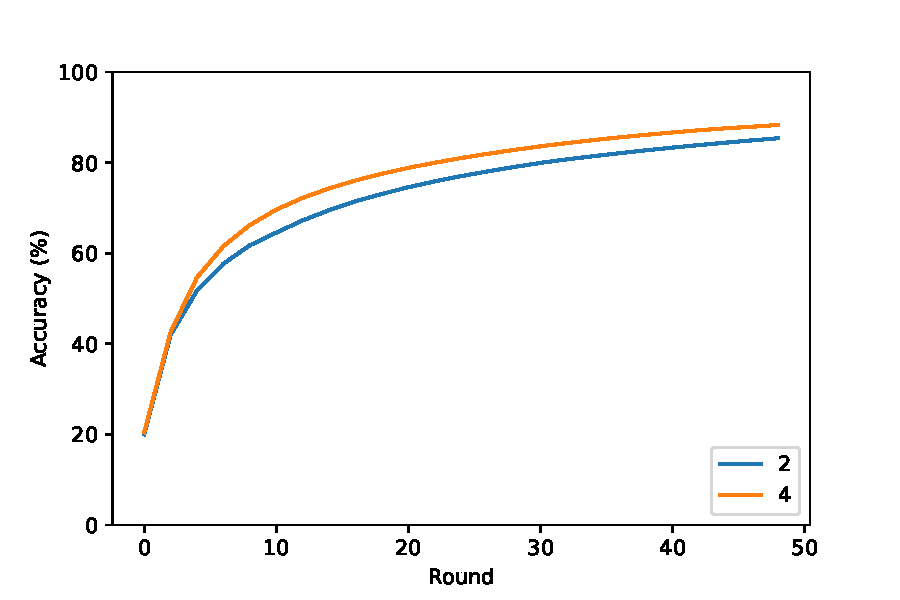
\includegraphics[width=0.7\textwidth]{graphics/vertical/accuracy.pdf}
    \caption{Accuracy Per Training Clients}
    \label{fig:accuracy_vertical}
\end{figure}

\section{Communication Costs}

\begin{figure}[!ht]
    \centering
    \centering
    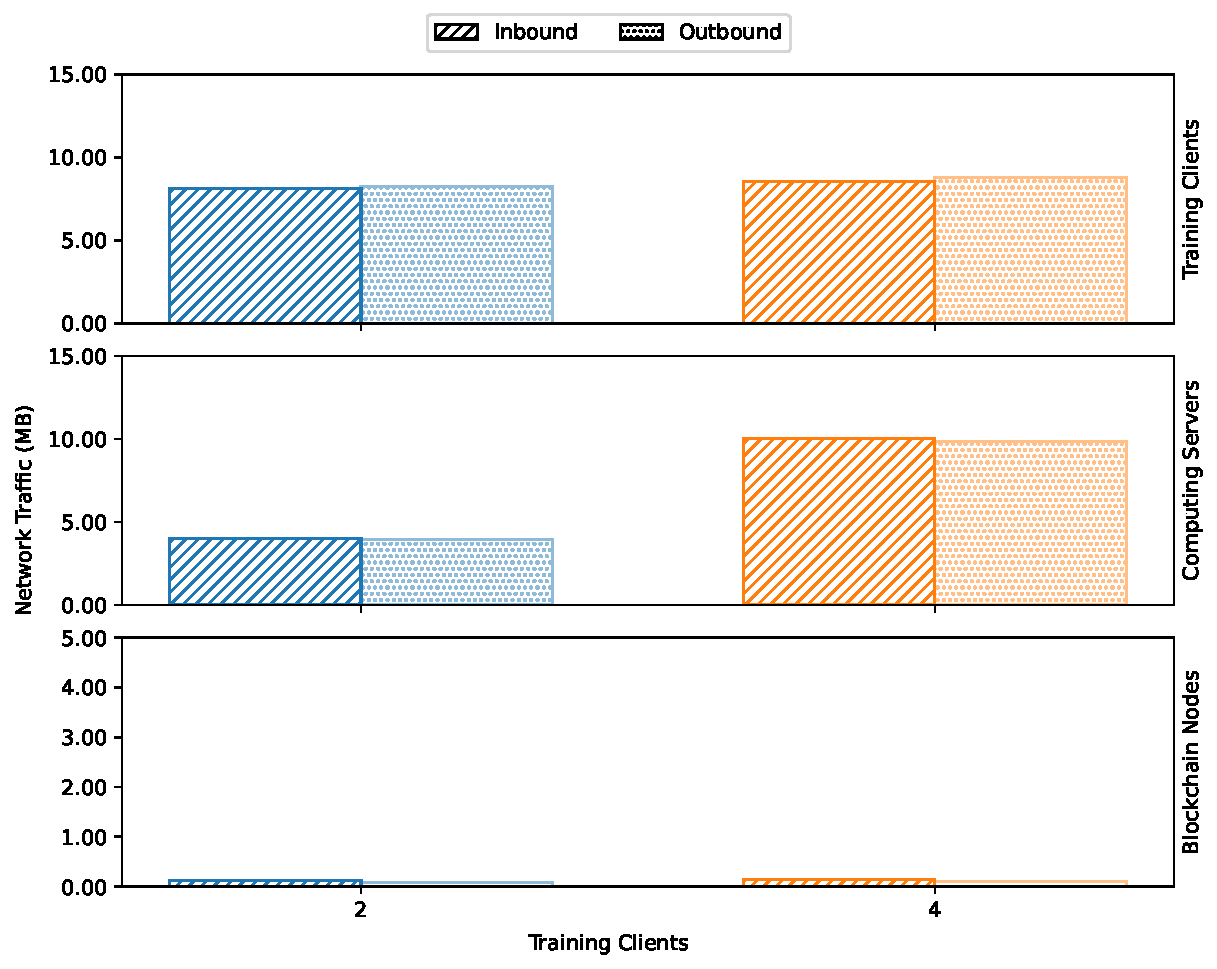
\includegraphics[width=0.8\textwidth]{graphics/vertical/net.pdf}
    \caption{Network Traffic Per Round Per Training Clients}
    \label{fig:net_vertical}
\end{figure}

\section{Computation Costs}

\begin{figure}[!hpt]
    \centering
    \centering
    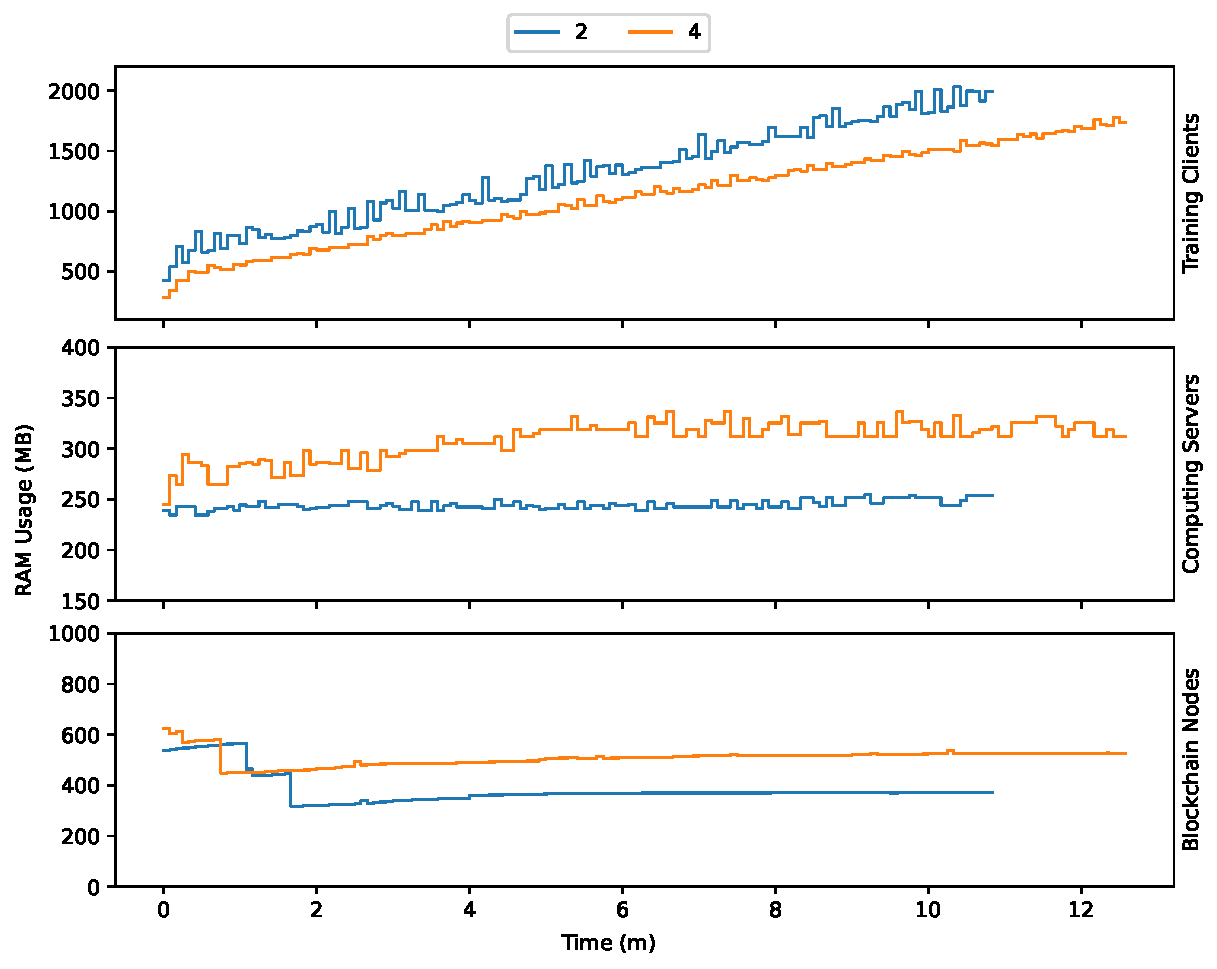
\includegraphics[width=0.8\textwidth]{graphics/vertical/ram.pdf}
    \caption{RAM Usage Per Training Clients}
    \label{fig:ram_vertical}
\end{figure}

\begin{figure}[!hpb]
    \centering
    \centering
    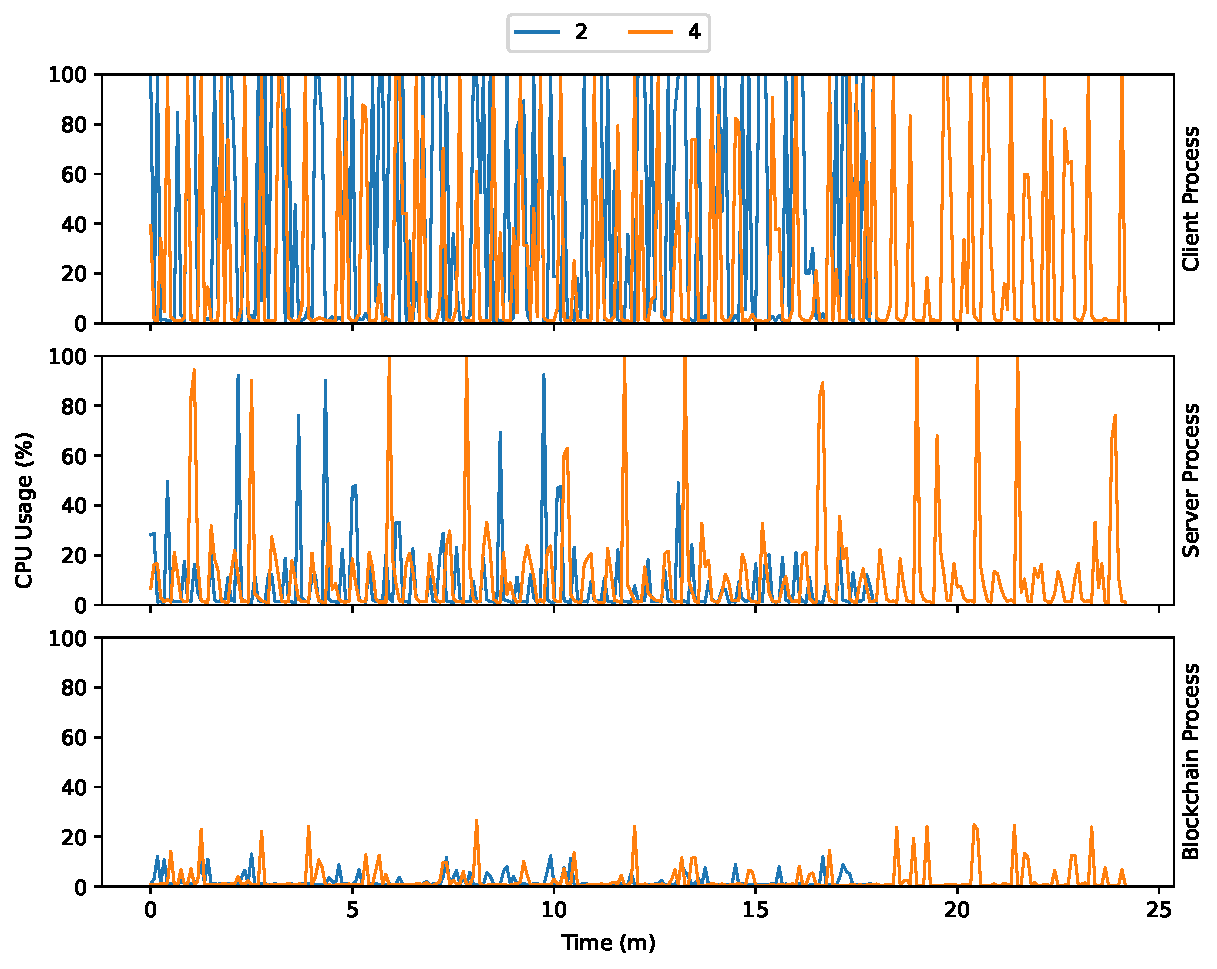
\includegraphics[width=0.8\textwidth]{graphics/vertical/cpu.pdf}
    \caption{CPU Usage Per Training Clients}
    \label{fig:cpu_vertical}
\end{figure}

\section{Conclusions} % and improvements? and limitations?
